\documentclass{article}

\usepackage{graphicx}
\usepackage{tikz}
\usepackage{tikzsymbols}
\usetikzlibrary{calc,patterns,shapes.geometric}
\pagestyle{empty}
\usepackage[margin=0pt]{geometry}
\geometry{papersize={14in,12in}}

\def\centerarc[#1](#2)(#3:#4:#5){\draw[#1] ($(#2)+({#5*cos(#3)},{#5*sin(#3)})$) arc (#3:#4:#5);}

\begin{document}
	\begin{figure}
		\centering
		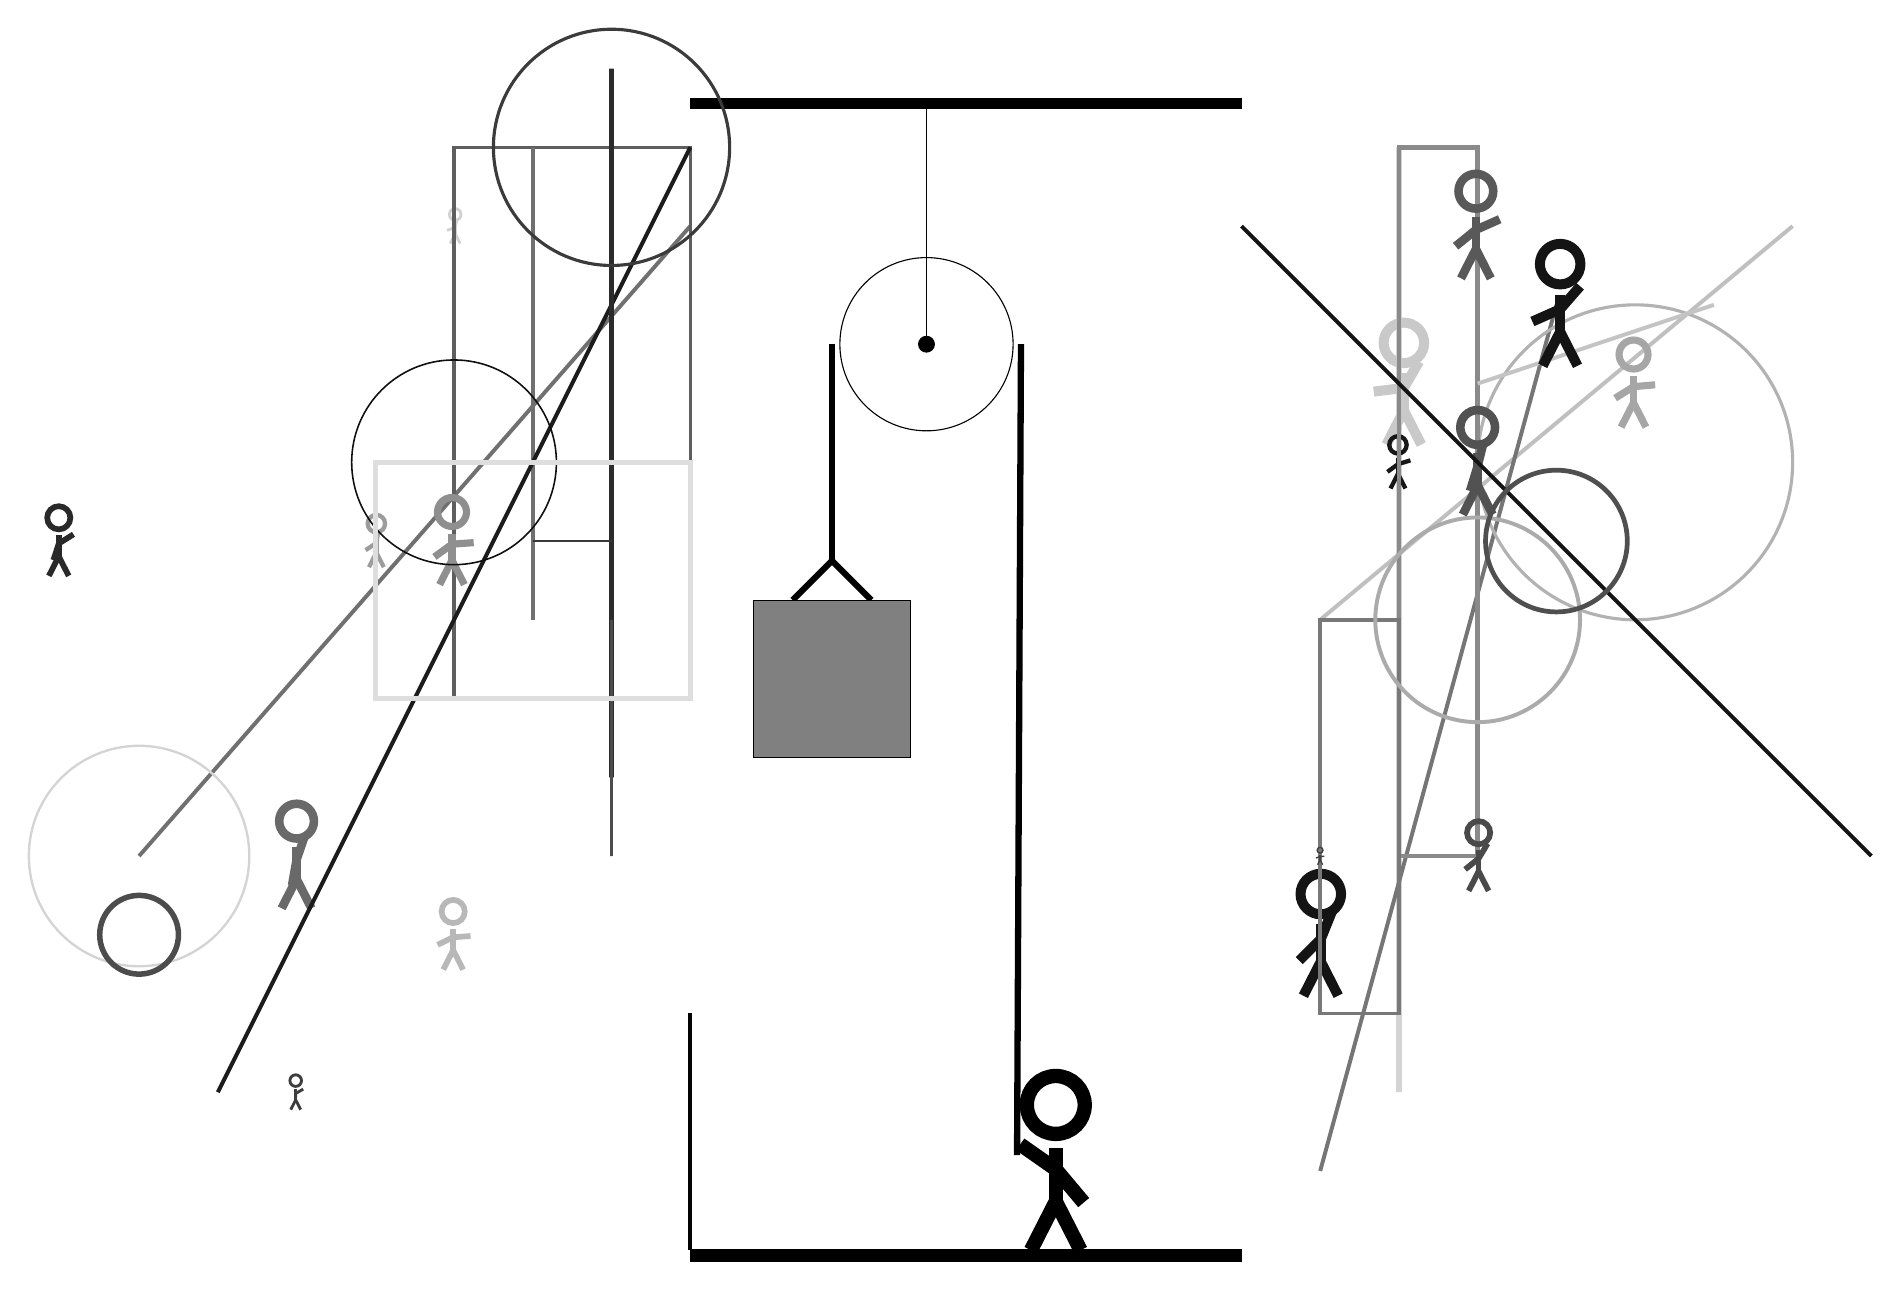
\begin{tikzpicture}
			%%%%% START %%%%%
			
			\draw[fill=black] (-2, 11.5) rectangle (5, 11.625);
			
			\draw (1, 8.5) circle (1.1);
			\draw[fill=black] (1, 8.5) circle (0.1);
			\draw (1, 11.5) -- (1, 8.5);
			
			\draw[line width=0.8mm] (-0.7, 5.25) -- (-0.2, 5.75) -- (0.3, 5.25);
			\draw[fill=black!50] (-1.2, 5.25) rectangle (0.8, 3.25);
			
			\draw[line width=0.8mm] (-0.2, 8.5) -- (-0.2, 5.75);
			\centerarc[line width=0.8mm](1, 8.5)(0:180:1.2000000000000002);
			\draw[line width=0.8mm](2.2, 8.5) -- (2.15, -1.8);
			
			\draw[line width=0.7mm, color=black!17] (7, 11) rectangle (7, -1);
			
			\node[line width=0.3mm, color=black!18] at (-5, 10) {\Strichmaxerl[2][21][78]};
			\node[line width=0.6mm, color=black!59] at (-7, 2) {\Strichmaxerl[6][80][71]};
			\node[line width=0.4mm, color=black!21] at (7, 8) {\Strichmaxerl[7][7][60]};
			\draw[line width=0.5mm, color=black!56](-2, 10) -- (-9, 2);
			\draw[line width=0.5mm, color=black!25](6, 5) -- (12, 10);
			
			\draw[line width=0.4mm, color=black!63] (-2, 4) rectangle (-5, 11);
			\draw[line width=0.5mm, color=black!54](9, 9) -- (6, -2);
			\draw [line width=0.3mm, color=black!17](-9, 2) circle (1.4);
			
			\node[line width=0.2mm, color=black!92] at (6, 1) {\Strichmaxerl[7][45][68]};
			
			\draw[line width=0.4mm, color=black!85] (-4, 8) rectangle (-4, 9);
			\draw [line width=0.4mm, color=black!30](10, 7) circle (2.0);
			\node[line width=0.3mm, color=black!44] at (-5, 6) {\Strichmaxerl[5][36][4]};
			\draw[line width=0.5mm, color=black!56] (-4, 11) rectangle (-4, 5);
			\node[line width=0.3mm, color=black!91] at (7, 7) {\Strichmaxerl[3][36][17]};
			\draw[line width=0.5mm, color=black!89](-2, 11) -- (-8, -1);
			
			\draw[line width=0.6mm, color=black!46] (7, 11) rectangle (8, 2);
			\draw[line width=0.5mm, color=black!53] (6, 0) rectangle (7, 5);
			\node[line width=0.7mm, color=black!74] at (6, 2) {\Strichmaxerl[1][18][5]};
			\draw [line width=0.7mm, color=black!70](-9, 1) circle (0.5);
			\node[line width=0.7mm, color=black!68] at (8, 7) {\Strichmaxerl[6][73][76]};
			
			\node[line width=0.7mm, color=black!35] at (10, 8) {\Strichmaxerl[5][32][5]};
			
			\node[line width=0.6mm, color=black!76] at (-7, -1) {\Strichmaxerl[2][88][30]};
			\draw[line width=0.6mm, color=black!83] (-3, 12) rectangle (-3, 3);
			\node[line width=0.5mm, color=black!39] at (-6, 6) {\Strichmaxerl[3][34][81]};
			
			\draw [line width=0.5mm, color=black!33](8, 5) circle (1.3);
			\draw [line width=0.2mm, color=black!94](-5, 7) circle (1.3);
			\node[line width=0.6mm, color=black!65] at (8, 10) {\Strichmaxerl[6][39][24]};
			\draw[line width=0.5mm, color=black!92](5, 10) -- (13, 2);
			
			\draw[line width=0.5mm, color=black!23](8, 8) -- (11, 9);
			\draw [line width=0.4mm, color=black!77](-3, 11) circle (1.5);
			\draw[line width=0.5mm, color=black!99](-2, 0) -- (-2, -3);
			\draw[line width=0.3mm, color=black!78] (-3, 6) rectangle (-4, 6);
			\draw [line width=0.6mm, color=black!69](9, 6) circle (0.9);
			\node[line width=0.2mm, color=black!84] at (-10, 6) {\Strichmaxerl[4][72][32]};
			\node[line width=0.6mm, color=black!92] at (9, 9) {\Strichmaxerl[7][24][49]};
			\draw[line width=0.3mm, color=black!70] (-3, 2) rectangle (-3, 5);
			
			\node[line width=0.7mm, color=black!28] at (-5, 1) {\Strichmaxerl[4][26][4]};
			\node[line width=0.4mm, color=black!71] at (8, 2) {\Strichmaxerl[4][39][59]};
			\draw[line width=0.6mm, color=black!13] (-2, 7) rectangle (-6, 4);
			
			\node at (2.6, -1.9) {\Strichmaxerl[10][-35][-50]};
			
			\draw[fill=black] (-2, -3) rectangle (5, -3.15);
			
			%%%%% END %%%%%
		\end{tikzpicture}
	\end{figure}	
\end{document}